\documentclass[9pt]{article}

\usepackage[utf8]{inputenc}
\usepackage[T1]{fontenc}
\usepackage[spanish,es-tabla]{babel}

\usepackage{geometry}
\geometry{
    a4paper,
    top=1.7cm,
    bottom=1.7cm,
    left=1.8cm,
    right=1.8cm
}

\usepackage{graphicx}
\graphicspath{{./}}
\usepackage{booktabs}
\usepackage{array}
\usepackage{enumitem}
\usepackage{xcolor}
\usepackage{tcolorbox}
\usepackage{hyperref}
\usepackage{titlesec}
\usepackage{fancyhdr}
\usepackage{float}
\usepackage{caption}

\definecolor{primaryblue}{RGB}{28,58,92}
\definecolor{accentblue}{RGB}{47,109,161}
\definecolor{lightgray}{RGB}{245,246,248}
\definecolor{midgray}{RGB}{100,100,100}
\definecolor{warningorange}{RGB}{180,105,20}

\setlength{\parindent}{0pt}
\setlength{\parskip}{3pt}

\setlist[itemize]{
    leftmargin=1.4em,
    itemsep=0pt,
    topsep=2pt
}

\setlist[enumerate]{
    leftmargin=1.5em,
    itemsep=0pt,
    topsep=2pt
}

\captionsetup{
    font=footnotesize,
    skip=2pt
}

\titleformat{\section}
{\normalsize\bfseries\color{primaryblue}}
{\thesection.}{0.35em}{}

\titlespacing*{\section}
{0pt}{7pt}{3pt}

\titleformat{\subsection}
{\small\bfseries\color{accentblue}}
{\thesubsection}{0.35em}{}

\titlespacing*{\subsection}
{0pt}{5pt}{2pt}

\pagestyle{fancy}
\fancyhf{}
\fancyhead[L]{\footnotesize\color{midgray} Recomendación local de citas académicas}
\fancyhead[R]{\footnotesize\color{midgray} Entrega 3}
\fancyfoot[C]{\footnotesize\color{midgray}\thepage}
\renewcommand{\headrulewidth}{0.3pt}

\hypersetup{
    colorlinks=true,
    linkcolor=accentblue,
    urlcolor=accentblue,
    pdftitle={Recomendación local de citas académicas - Entrega 3}
}

\newcommand{\notabox}[1]{
\begin{tcolorbox}[
    colback=lightgray,
    colframe=accentblue,
    boxrule=0.5pt,
    left=5pt,
    right=5pt,
    top=3pt,
    bottom=3pt,
    arc=1pt
]
\footnotesize #1
\end{tcolorbox}
}

\newcommand{\pendingbox}[1]{
\begin{tcolorbox}[
    colback=orange!5,
    colframe=warningorange,
    boxrule=0.5pt,
    left=5pt,
    right=5pt,
    top=3pt,
    bottom=3pt,
    arc=1pt
]
\footnotesize #1
\end{tcolorbox}
}

\begin{document}

% ============================================================================
% CABECERA
% ============================================================================

\begin{center}

{\Large\bfseries\color{primaryblue}
Recomendación local de citas académicas mediante aprendizaje automático
}

\vspace{2pt}

{\normalsize
Reporte final -- Entrega 3
}

\vspace{3pt}

\footnotesize
Maestría en Inteligencia Artificial -- Universidad de los Andes

Carlos Duque · Carlos Caicedo · José Zambrana · John Arias

Proyecto: Desarrollo de Soluciones

22 de septiembre de 2026

\vspace{3pt}
{\color{primaryblue}\rule{\linewidth}{0.7pt}}

\end{center}

% ============================================================================
% 1. PROBLEMA Y DATOS
% ============================================================================

\section{Problema, datos y alcance}

Encontrar una referencia adecuada para respaldar una afirmación académica puede
convertirse en una tarea costosa cuando el autor debe buscar entre miles de
publicaciones relacionadas con un mismo tema. La recomendación local de citas
busca reducir ese esfuerzo utilizando como punto de partida el fragmento de
texto en el que se necesita incorporar una referencia.

Este problema ha sido abordado mediante modelos que utilizan el contexto local
de la cita para recuperar y ordenar artículos relevantes. En particular, Gu,
Gao y Hahnloser (2022) proponen una arquitectura de recomendación local de citas
que combina recuperación y reordenamiento de candidatos.

\notabox{
\textbf{Pregunta de negocio:}
¿Cómo apoyar a un autor de textos académicos en la identificación de artículos
potencialmente relevantes para citar utilizando el contexto textual local?
}

El prototipo desarrollado recibe un fragmento académico en inglés y devuelve
una lista ordenada de artículos candidatos. Para cada resultado se presentan
el identificador del documento, el título, el resumen y las puntuaciones
utilizadas por el recomendador.

El proyecto trabaja con el conjunto \texttt{custom} (ACL-200), proveniente del
repositorio \textit{Local-Citation-Recommendation} publicado por Gu (2022).
El corpus utilizado contiene 63.768 contextos de cita y 19.776 artículos
candidatos. Las particiones empleadas incluyen 30.390 consultas de entrenamiento,
9.381 de validación y 9.585 de prueba.

Los archivos de datos se administran con DVC a través de
\texttt{data/raw.dvc} y \texttt{data/processed.dvc}. De esta forma, Git se
mantiene enfocado en el código, la configuración y la documentación, mientras
DVC conserva el versionamiento de los conjuntos utilizados durante los
experimentos.

% ============================================================================
% 2. ARQUITECTURA
% ============================================================================

\section{Arquitectura y modelo}

La solución se organizó en dos etapas. Primero, TF--IDF recupera los artículos
más parecidos al contexto de consulta. Después, un modelo supervisado vuelve a
ordenar esos candidatos para intentar ubicar la cita correcta entre las primeras
posiciones.

\begin{center}
\footnotesize
Contexto
$\rightarrow$
TF--IDF
$\rightarrow$
Top--100
$\rightarrow$
reordenador lineal
$\rightarrow$
Top--K
$\rightarrow$
wheel \texttt{modelo-citas}
$\rightarrow$
FastAPI
$\rightarrow$
Nginx/tablero
\end{center}

La primera etapa compara el contexto con los 19.776 artículos del corpus
mediante similitud coseno y conserva los 100 candidatos con mayor puntaje.

Sobre esos candidatos se aplica una regresión logística que utiliza cinco
características:

\begin{itemize}
    \item similitud TF--IDF entre el contexto y el título;
    \item similitud TF--IDF entre el contexto y el resumen;
    \item longitud del contexto;
    \item longitud del título;
    \item longitud del resumen.
\end{itemize}

Para entrenar el reordenador se construyeron aproximadamente 91.170 pares
contexto--artículo. Cada consulta aporta una cita positiva y dos ejemplos
negativos.

Se probaron dos formas de seleccionar esos negativos. En la primera,
\texttt{random}, los artículos incorrectos se escogen aleatoriamente. En la
segunda, \texttt{hard}, se utilizan artículos incorrectos que TF--IDF considera
muy parecidos al contexto.

Las siguientes capturas corresponden a las ejecuciones utilizadas para entrenar
ambas variantes.

\begin{figure}[H]
\centering

\begin{minipage}{0.49\textwidth}
\centering
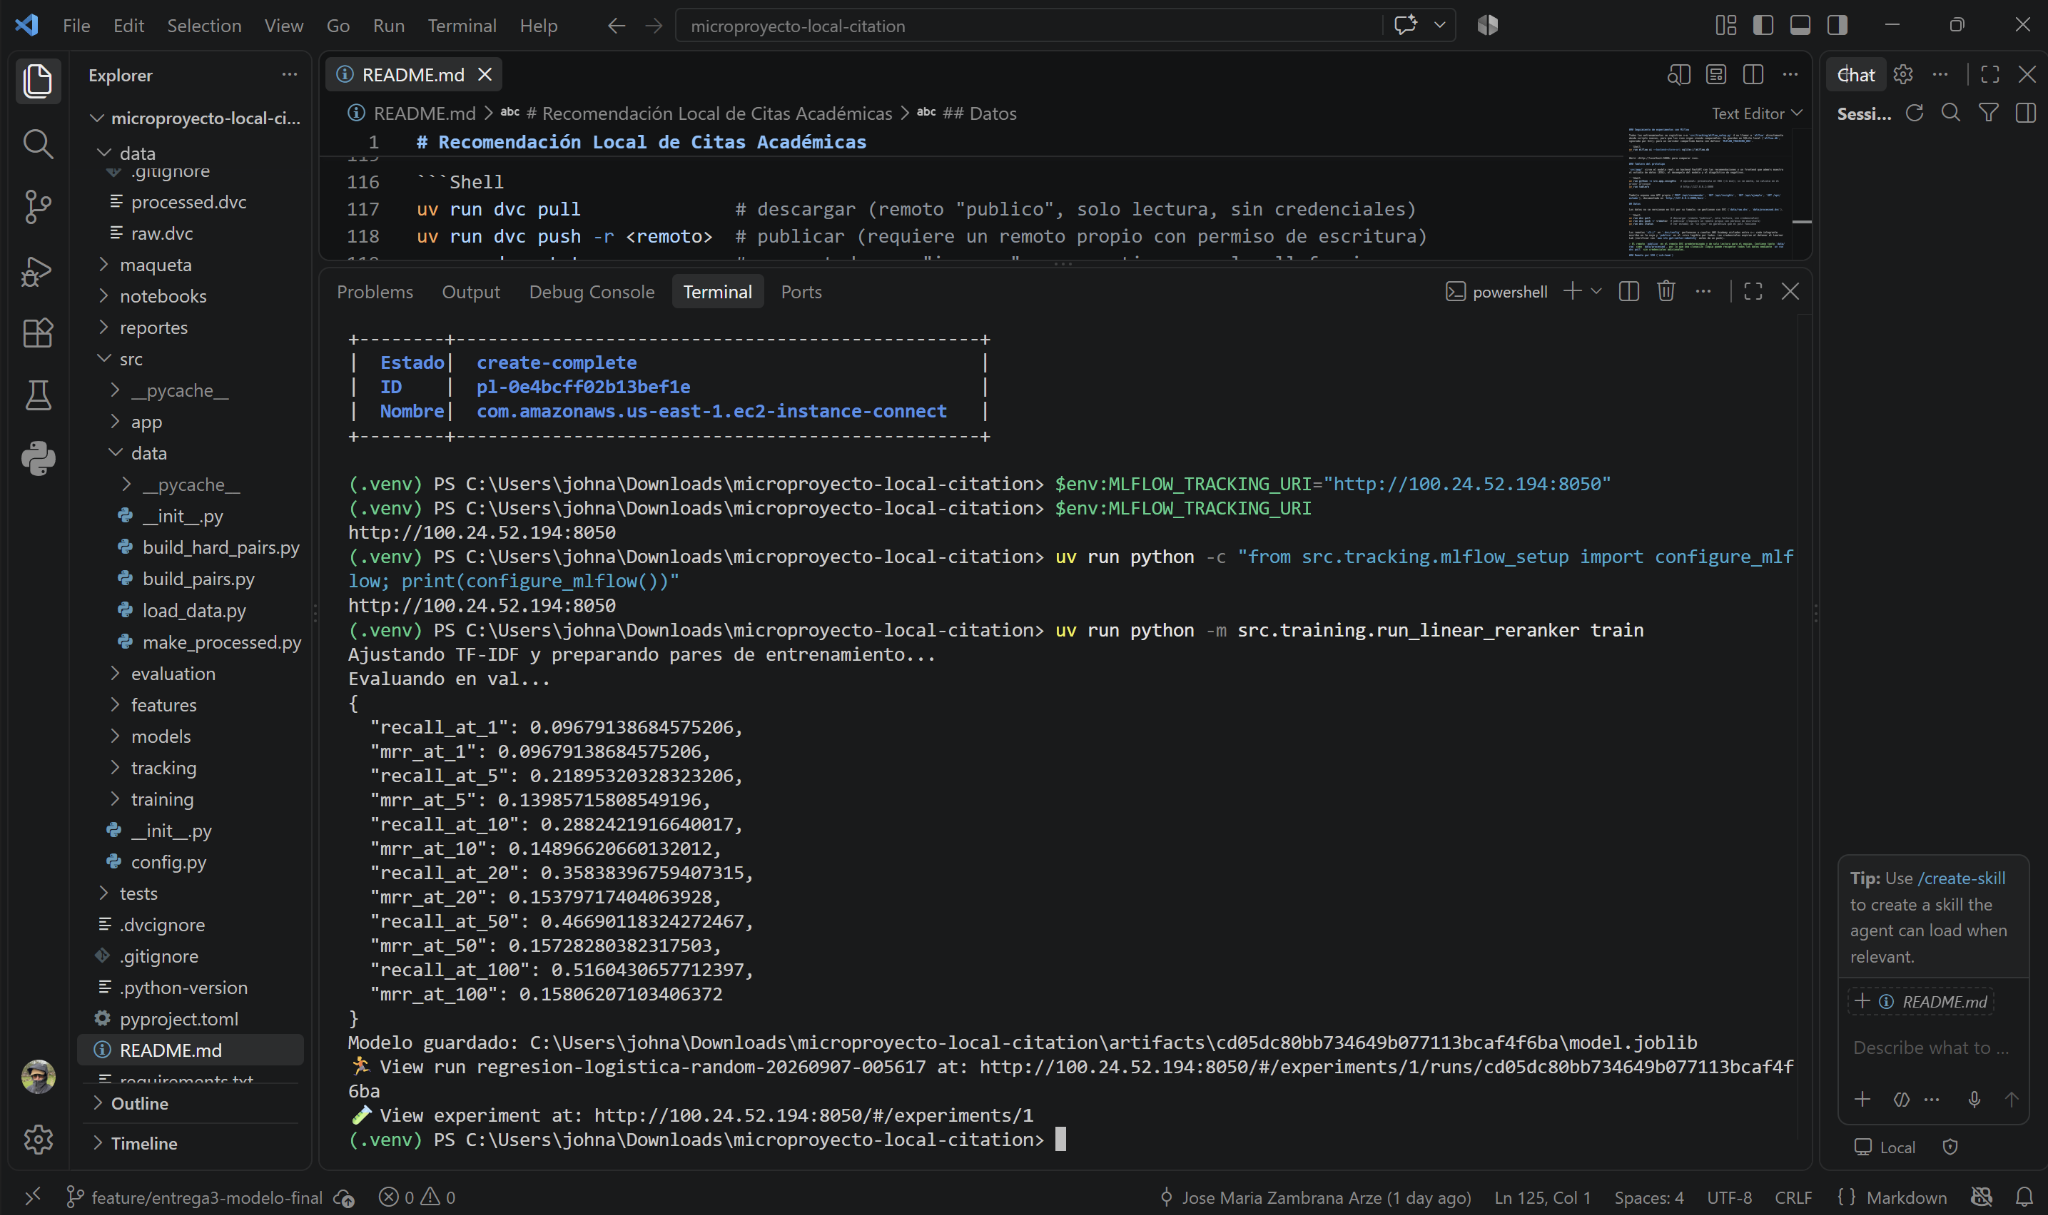
\includegraphics[width=\linewidth]{entrenamiento_random_terminal.png}
\caption*{(a) Entrenamiento con negativos aleatorios}
\end{minipage}
\hfill
\begin{minipage}{0.49\textwidth}
\centering
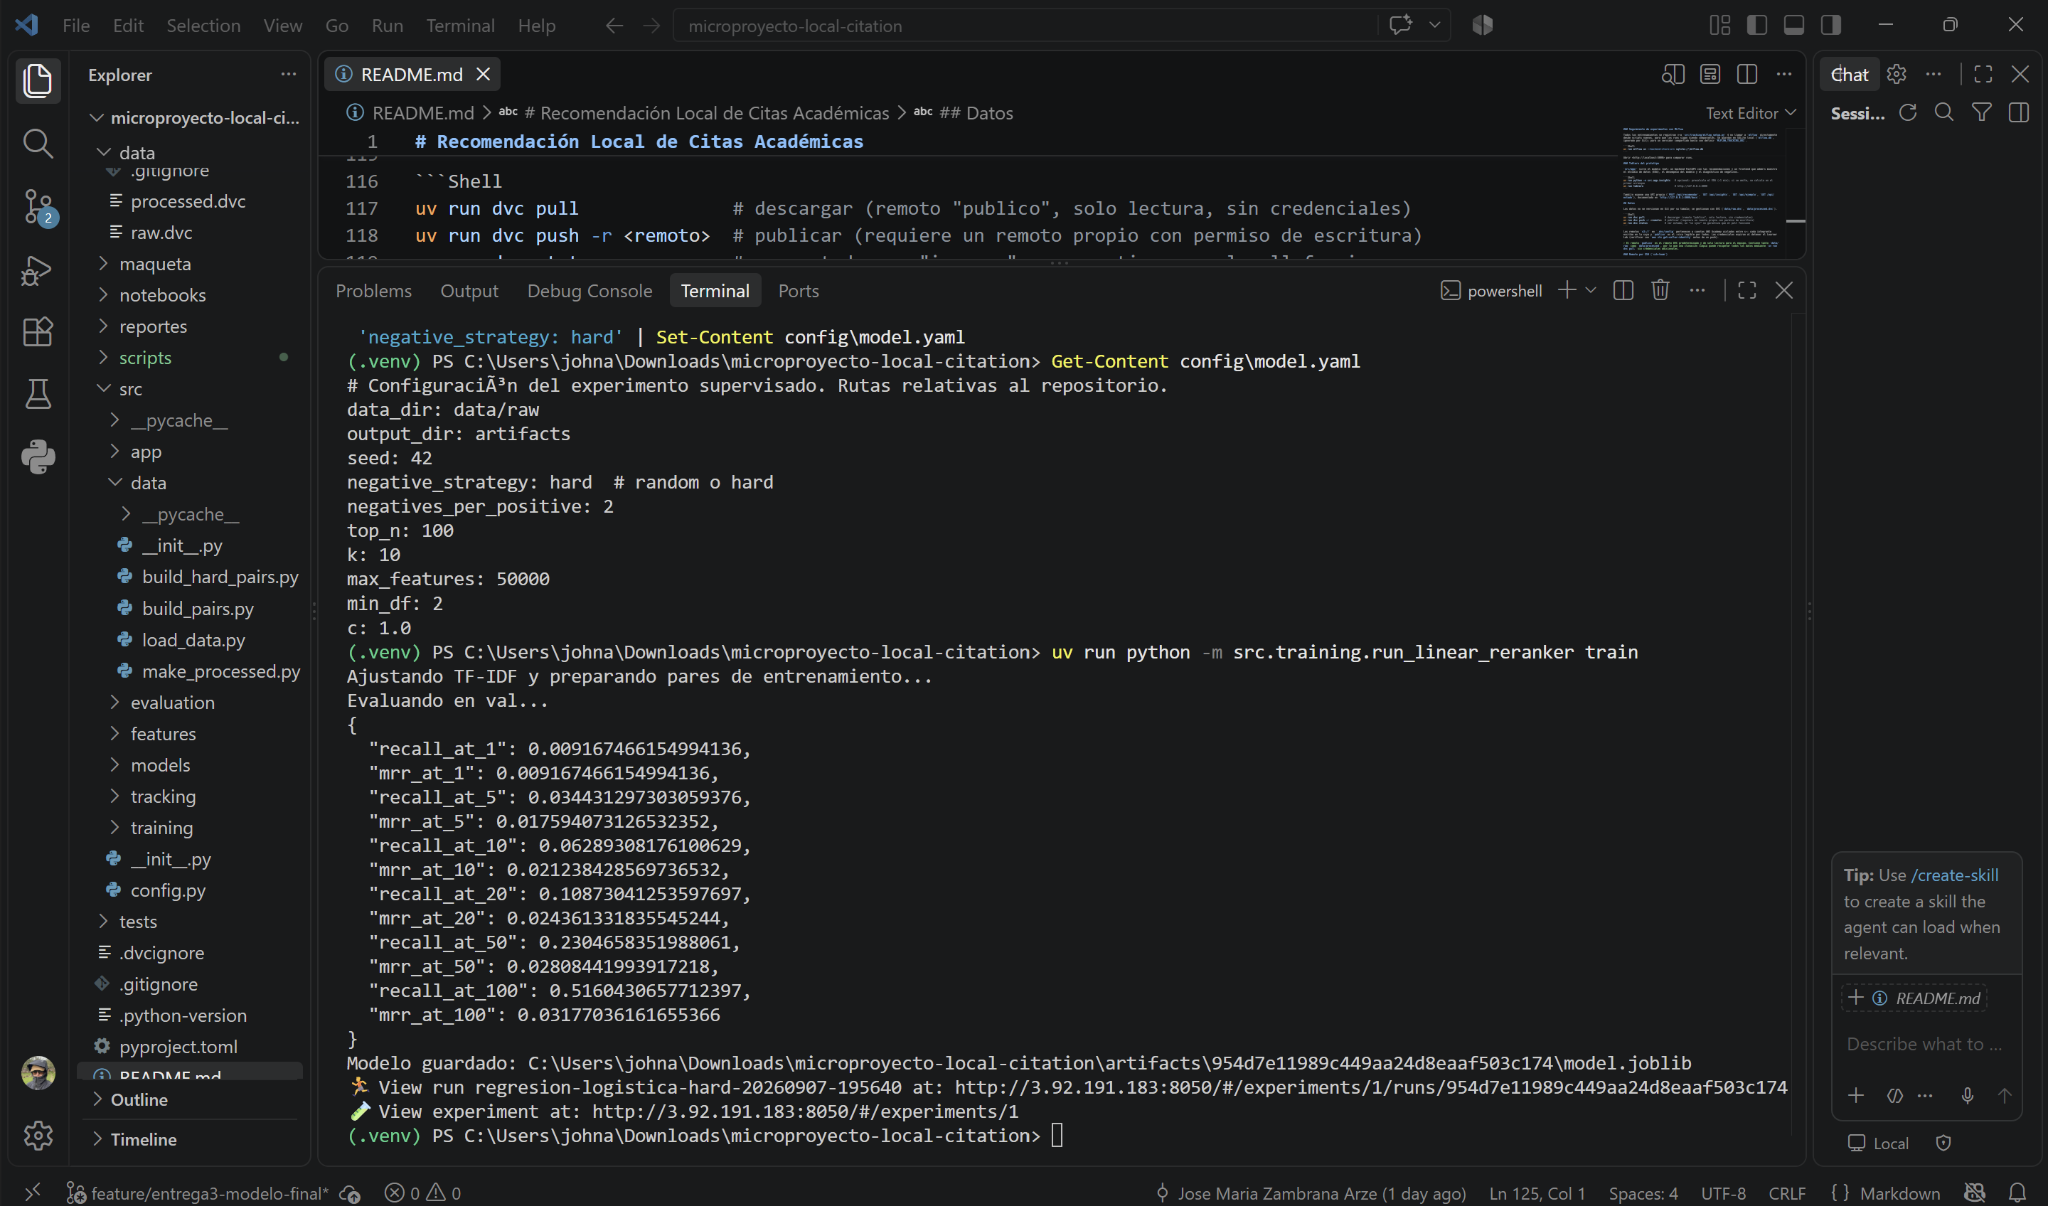
\includegraphics[width=\linewidth]{entrenamiento_hard_terminal.png}
\caption*{(b) Entrenamiento con negativos difíciles}
\end{minipage}

\caption{Evidencias de entrenamiento de las dos estrategias evaluadas.}
\end{figure}

% ============================================================================
% 3. RESULTADOS
% ============================================================================

\section{Resultados experimentales}

Las dos variantes se evaluaron con las mismas particiones de datos, la misma
semilla y los mismos parámetros generales. La única diferencia controlada fue
la estrategia utilizada para seleccionar los ejemplos negativos.

Los resultados principales fueron los siguientes:

\begin{table}[H]
\centering
\footnotesize
\caption{Comparación de los modelos sobre las 9.381 consultas de validación}

\begin{tabular}{lccc}
\toprule
\textbf{Modelo} &
\textbf{Recall@10} &
\textbf{MRR@10} &
\textbf{Recall@100} \\
\midrule

TF--IDF sin reordenar &
0,2571 &
0,1339 &
0,5160 \\

v1 · Random &
0,2882 &
0,1490 &
0,5160 \\

v1 · Hard &
0,0629 &
0,0212 &
0,5160 \\

\textbf{v2 · Random} &
\textbf{0,3793} &
\textbf{0,2166} &
0,5160 \\

v2 · Hard &
0,2288 &
0,0995 &
0,5160 \\

\bottomrule
\end{tabular}
\end{table}

El \emph{Recall@100} se mantiene en 0,5160 en las cinco filas. Esa invariancia
comprueba que el reordenador opera efectivamente como segunda etapa --recibe el
mismo conjunto recuperado y solo altera el orden-- y marca a la vez el techo del
sistema: mientras la primera etapa no recupere el artículo correcto, ningún
reordenamiento puede corregirlo.

La línea base de comparación es 0,2571 / 0,1339 y no 0,2541 / 0,1249, porque
excluye el artículo citante igual que lo hace el conjunto de candidatos que
consume el reordenador. Compararlo contra la versión que sí lo incluye inflaría
la mejora atribuida al modelo.

En la primera versión (v1), la diferencia entre las dos estrategias es
considerable en las primeras posiciones del ranking. Con negativos aleatorios,
Recall@10 alcanza 0,2882, mientras que con negativos difíciles baja a 0,0629.
El mismo comportamiento aparece en MRR@10, que pasa de 0,1490 a 0,0212.

Las gráficas siguientes permiten observar esta diferencia de manera directa.

\begin{figure}[H]
\centering

\begin{minipage}{0.49\textwidth}
\centering
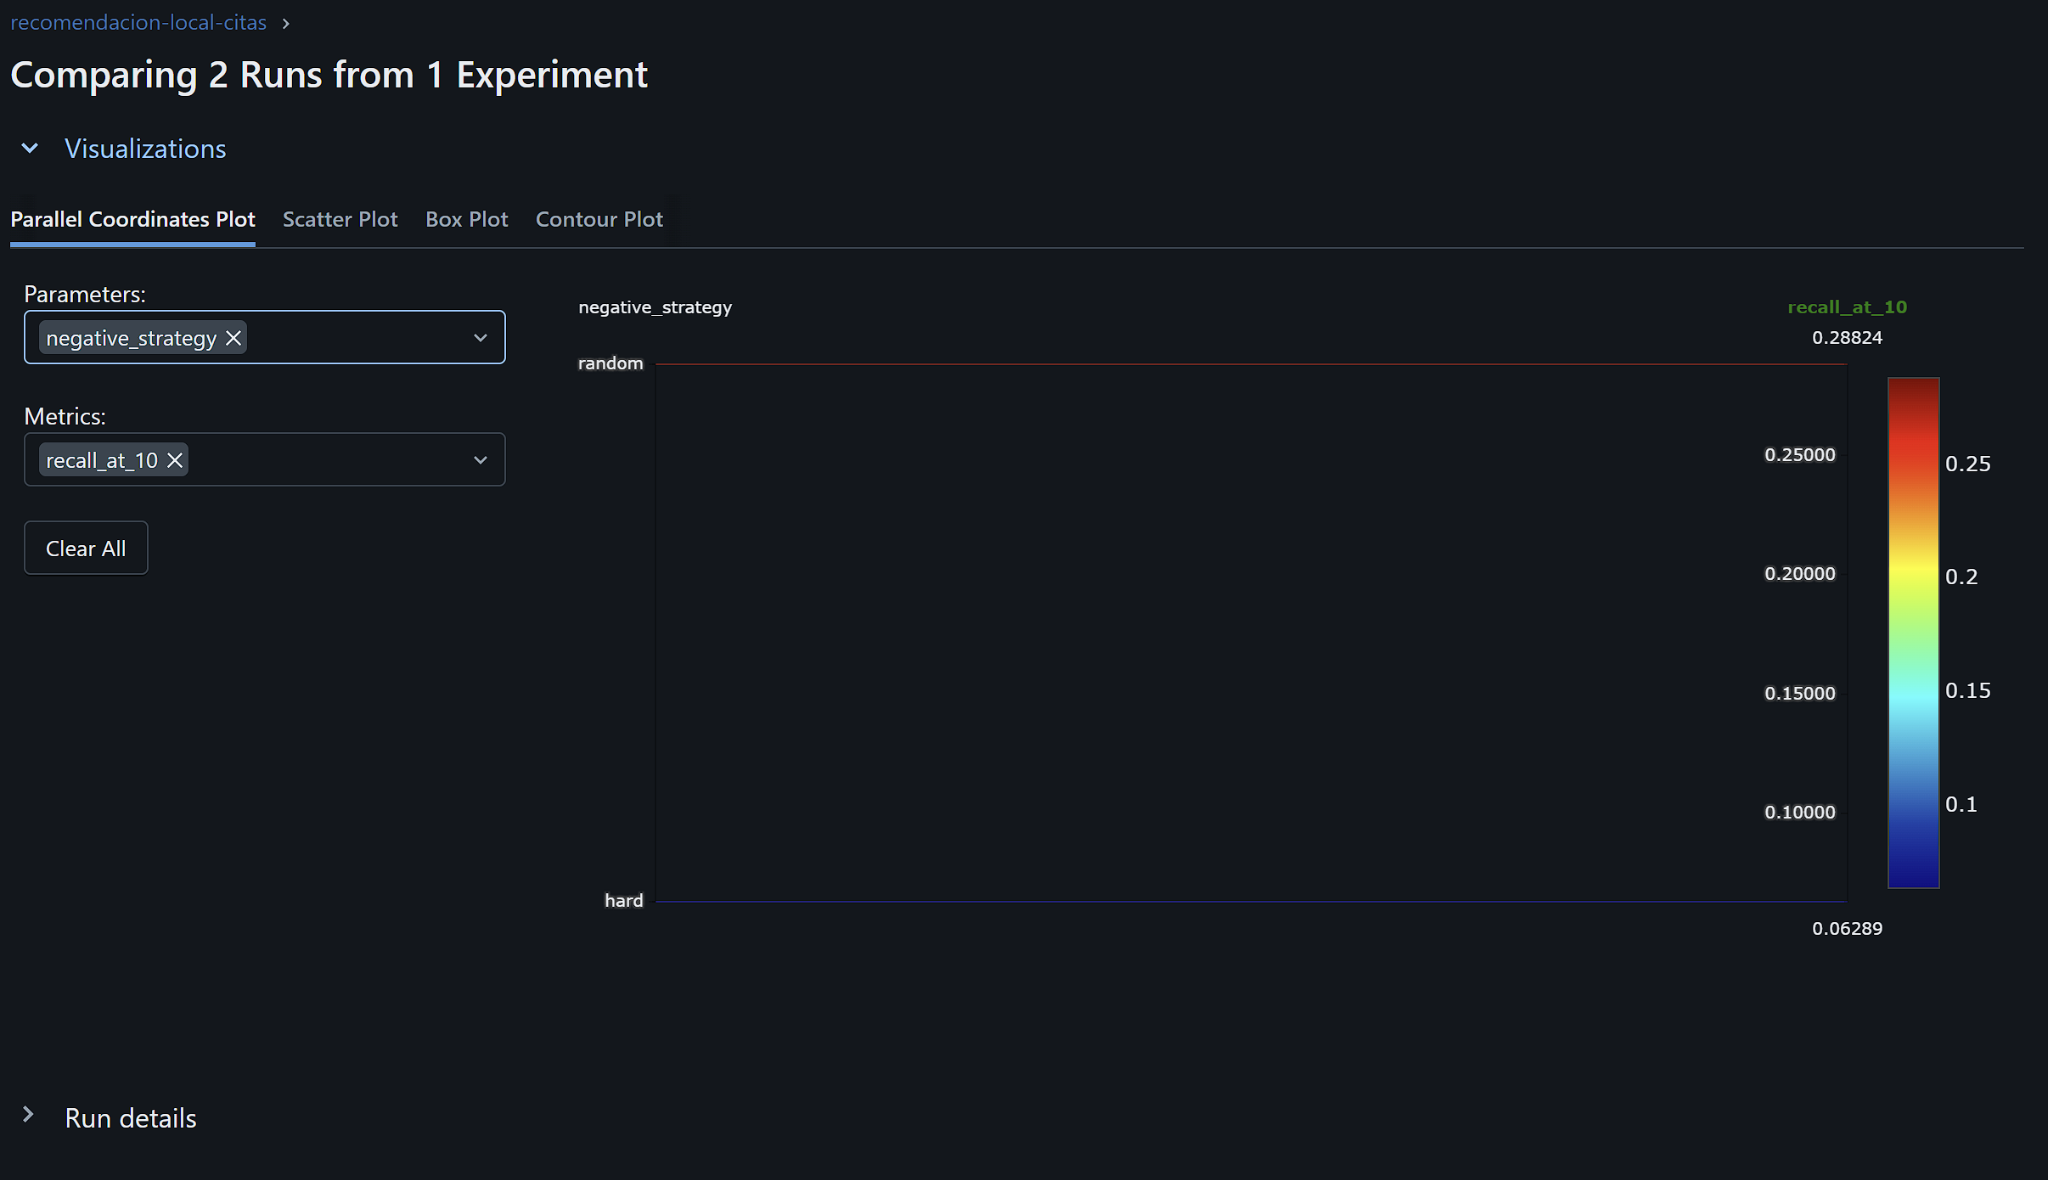
\includegraphics[width=\linewidth]{comparacion_random_hard_recall10.png}
\caption*{(a) Comparación de Recall@10}
\end{minipage}
\hfill
\begin{minipage}{0.49\textwidth}
\centering
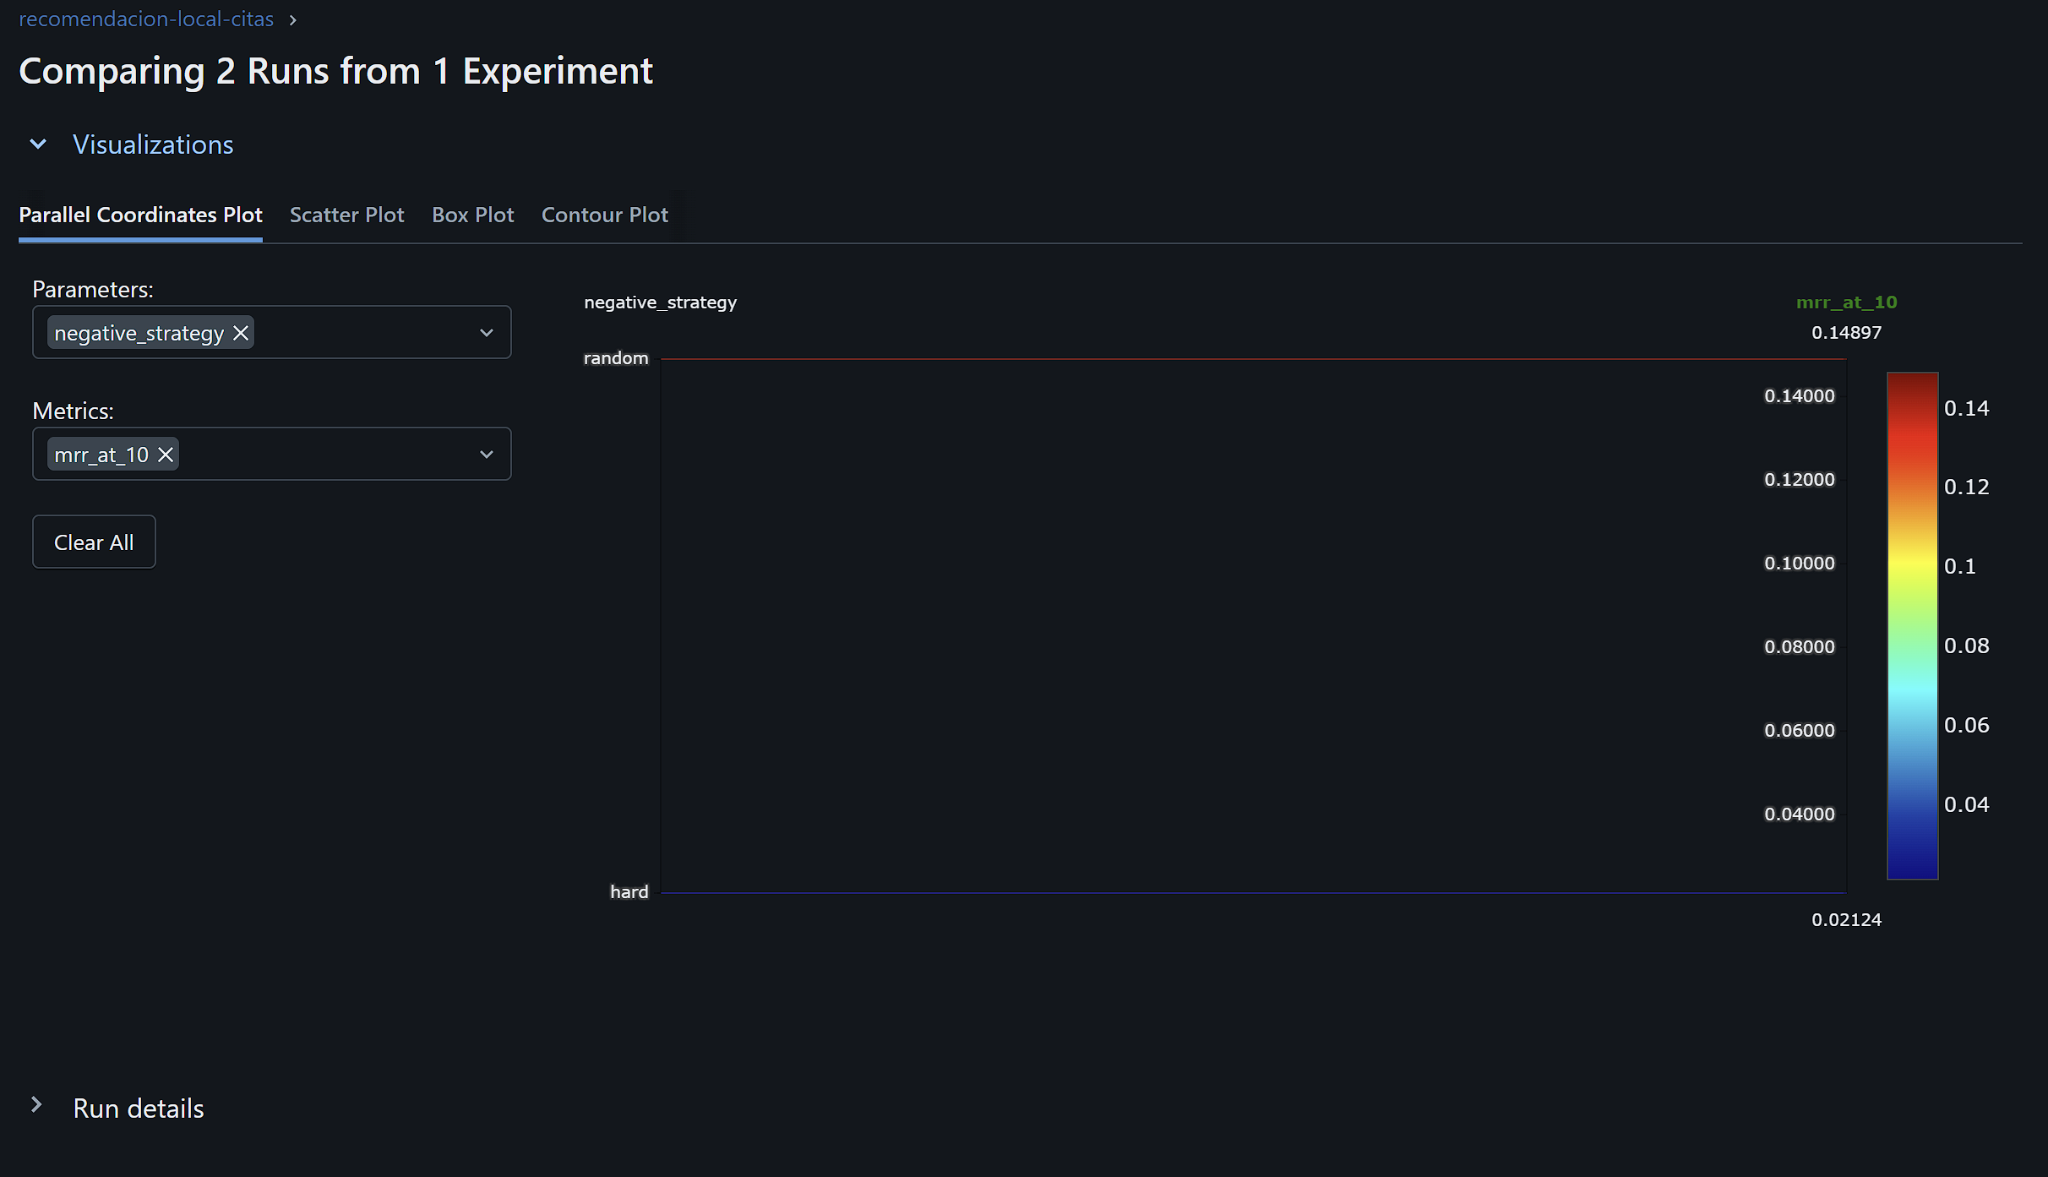
\includegraphics[width=\linewidth]{comparacion_random_hard_mrr10.png}
\caption*{(b) Comparación de MRR@10}
\end{minipage}

\caption{Desempeño de las estrategias Random y Hard en las primeras posiciones del ranking.}
\end{figure}

\subsection{Segunda versión: ampliación de las características}

La comparación anterior sugirió que una parte importante del cuello de botella
estaba en la representación disponible para el reordenador. Entrenado con
negativos difíciles, el modelo asignaba un coeficiente de $-2{,}09$ a la
similitud con el resumen. Ese signo es consistente con la señal observada en
este conjunto: el área bajo la curva ROC de positivos frente a negativos
difíciles usando solo similitud coseno es $0{,}4053$, por debajo de $0{,}5$.
Con únicamente cinco características léxicas, distinguir un positivo entre
candidatos ya muy parecidos resulta especialmente difícil.

La segunda versión amplía el vector a diez características. Las cinco nuevas se
derivan de los metadatos que codifica el identificador del ACL Anthology
--tipo de publicación, año y número, formato que cumplen los 19.776 artículos
del corpus-- y del conjunto de entrenamiento:

\begin{itemize}[leftmargin=1.4em, itemsep=1pt, topsep=2pt]
  \item \texttt{year\_diff}: años entre el artículo citante y el candidato.
  \item \texttt{is\_future}: candidato publicado después del citante, es decir
        una cita imposible.
  \item \texttt{same\_venue}: coincidencia en el tipo de publicación.
  \item \texttt{title\_overlap}: fracción del título presente en el contexto.
  \item \texttt{citation\_prior}: logaritmo de las veces que el candidato se
        cita en entrenamiento.
\end{itemize}

La señal temporal resultó especialmente útil. Antes de incorporarla, el
11,1\,\% de los cupos del \emph{Top}--100 correspondía a artículos posteriores
al citante. En las 9.381 consultas de validación no se observó ningún positivo
posterior al artículo citante; por tanto, en esa partición la señal permite
penalizar candidatos temporalmente incompatibles sin perder un positivo
observado.

Los coeficientes de la mejor variante experimental muestran el peso de estas
señales: sobre características estandarizadas, \texttt{is\_future} obtiene
$-3{,}0790$ y \texttt{citation\_prior} $+2{,}6889$, ambos con magnitud
comparable o superior a \texttt{similarity\_abstract} ($+2{,}4954$). La
regresión asigna así una penalización fuerte a los candidatos posteriores al
artículo citante, sin aplicar un filtro temporal determinista.

\medskip

La \textbf{mejor variante experimental es la versión 2 con negativos
aleatorios}, de acuerdo con las métricas de ranking: frente a la línea base
comparable mejora un 47,5\,\% en Recall@10 y un 61,8\,\% en MRR@10; frente a
la primera versión, un 31,6\,\% y un 45,4\,\%. La ganancia es mayor en MRR
que en Recall, un comportamiento coherente con una segunda etapa que reordena
candidatos ya recuperados.

Con el vector ampliado, la variante de negativos difíciles mejora 3,6 veces en
Recall@10 (de 0,0629 a 0,2288), aunque permanece por debajo de la variante
aleatoria. La suma de los coeficientes de similitud continúa siendo negativa, de
modo que las características nuevas compensan parte de esa señal. Aprovechar
mejor los negativos difíciles probablemente requiera una representación
semántica más rica, por ejemplo densa, además de las señales tabulares.

Recall@100 permanece alrededor de 0,516 en las dos configuraciones porque
ambas reciben exactamente los mismos 100 candidatos recuperados por TF--IDF.
Esto indica que la diferencia entre los experimentos se encuentra en el
ordenamiento y no en la recuperación inicial.

El resultado de la estrategia \texttt{hard} también permitió identificar una
limitación del modelo. Los negativos difíciles son artículos que ya presentan
una gran similitud léxica con el contexto y, utilizando únicamente cinco
características, el reordenador dispone de poca información adicional para
distinguirlos correctamente.

Por métricas se priorizó la estrategia \texttt{random}. Es importante
distinguir entre el mejor resultado experimental y la versión actualmente
servida: el wheel \texttt{modelo-citas} 0.2.0 validado en Docker conserva
\texttt{include\_metadata=false}, por lo que el modelo desplegado corresponde a
la versión 1 con negativos aleatorios y cinco características. Esa versión
obtuvo Recall@10 de 0,2882 y MRR@10 de 0,1490. La versión 2 queda documentada
como la mejor variante experimental y requiere publicarse en un nuevo wheel
para convertirse en la versión desplegada.

% ============================================================================
% 4. MLFLOW
% ============================================================================

\section{Seguimiento de experimentos con MLflow}

Para llevar un registro común de los experimentos realizados por el equipo, el
entrenamiento se integró con MLflow. Cada corrida conserva sus parámetros,
métricas de ranking, tiempos de procesamiento y artefactos asociados.

La configuración se centralizó en
\texttt{src/tracking/mlflow\_setup.py} para que todas las ejecuciones siguieran
la misma estructura de seguimiento.

Este tipo de organización es coherente con las prácticas de MLOps, en las que
se busca mantener trazabilidad sobre datos, experimentos, modelos y
configuraciones durante el desarrollo de una solución de aprendizaje automático
(Treveil \& Dataiku Team, 2021).

Las siguientes capturas muestran las corridas Random y Hard registradas en
MLflow y la comparación de sus tiempos de procesamiento.

\begin{figure}[H]
\centering

\begin{minipage}{0.49\textwidth}
\centering
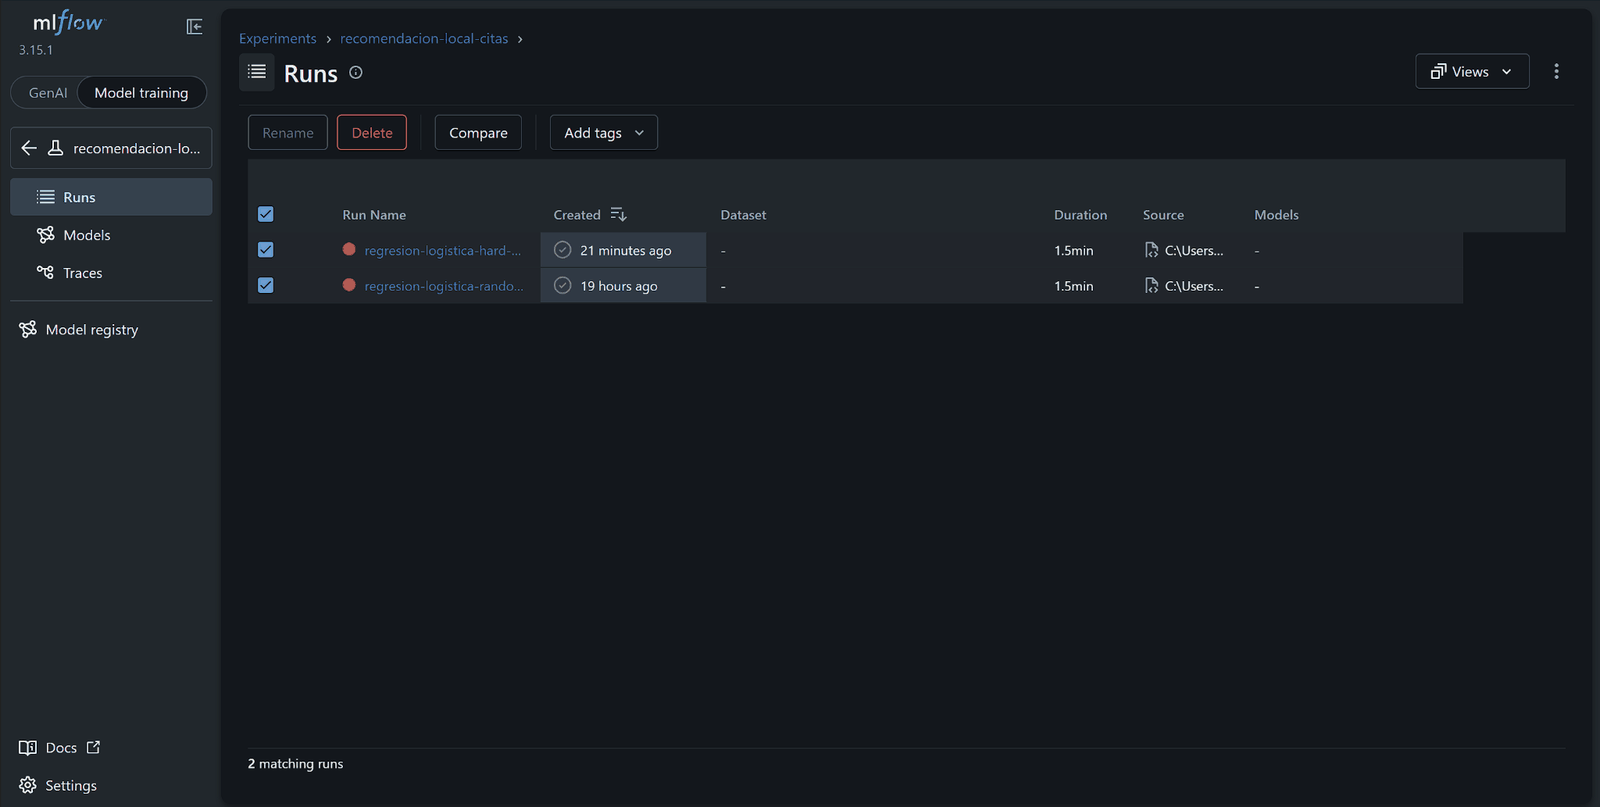
\includegraphics[width=\linewidth]{mlflow_runs_random_hard.png}
\caption*{(a) Corridas Random y Hard registradas en MLflow}
\end{minipage}
\hfill
\begin{minipage}{0.49\textwidth}
\centering
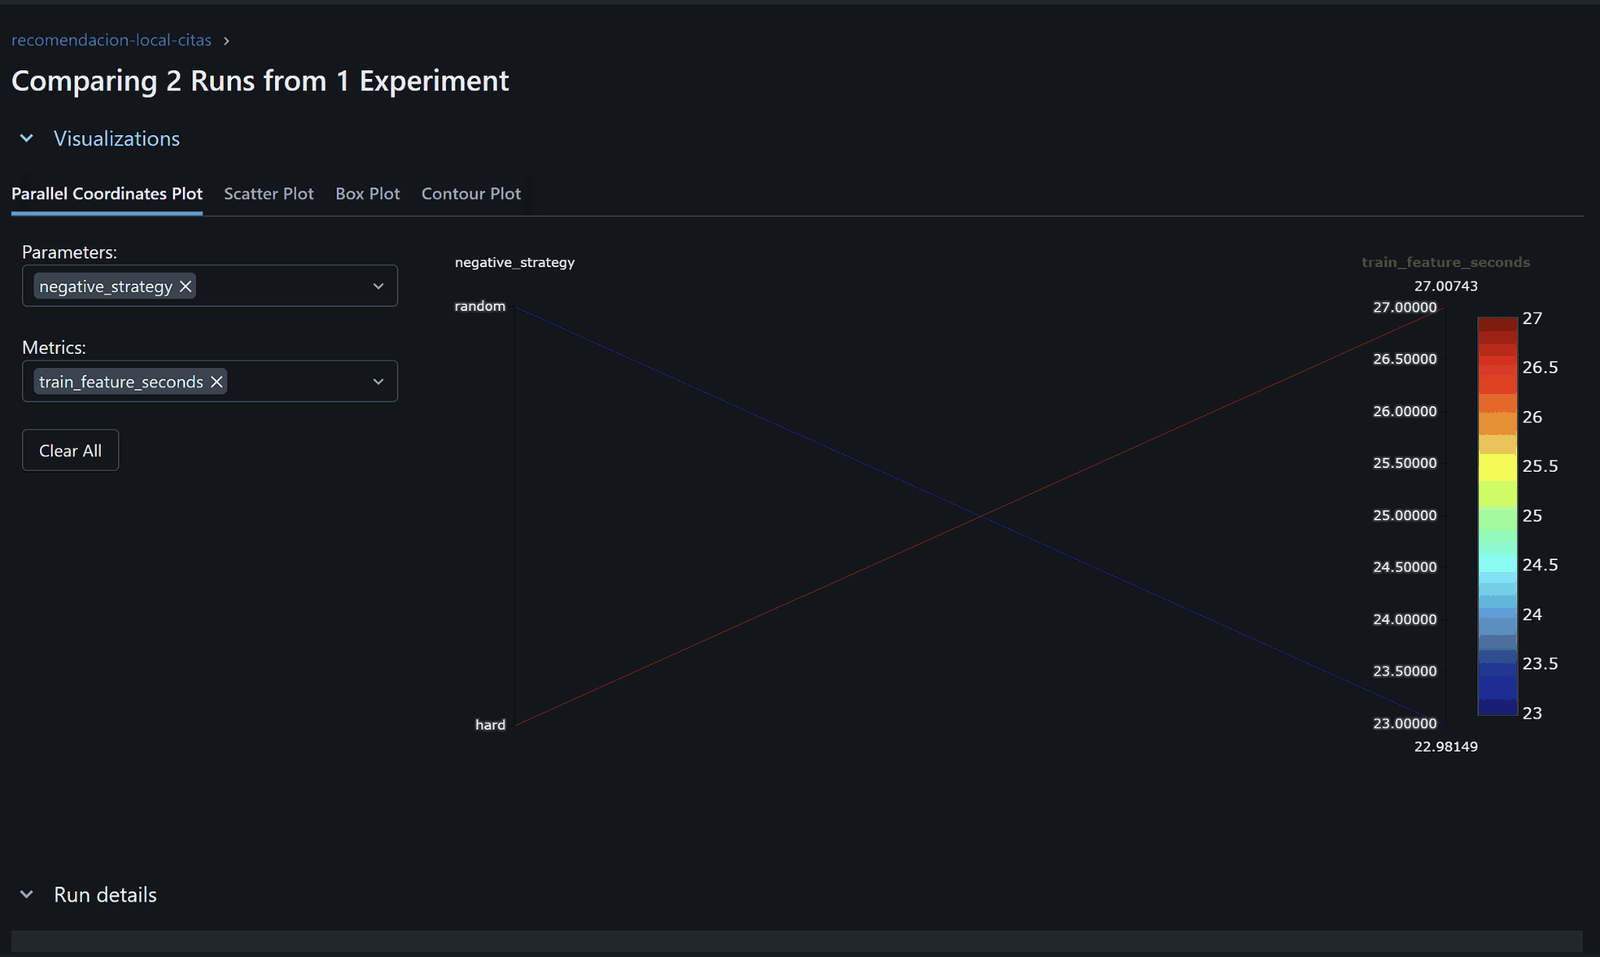
\includegraphics[width=\linewidth]{mlflow_comparacion_tiempo_features.png}
\caption*{(b) Comparación del tiempo de generación de características}
\end{minipage}

\caption{Seguimiento y comparación de los experimentos realizados.}
\end{figure}

Las siguientes capturas muestran el detalle de las métricas y los parámetros
guardados para cada ejecución.

\begin{figure}[H]
\centering

\begin{minipage}{0.49\textwidth}
\centering
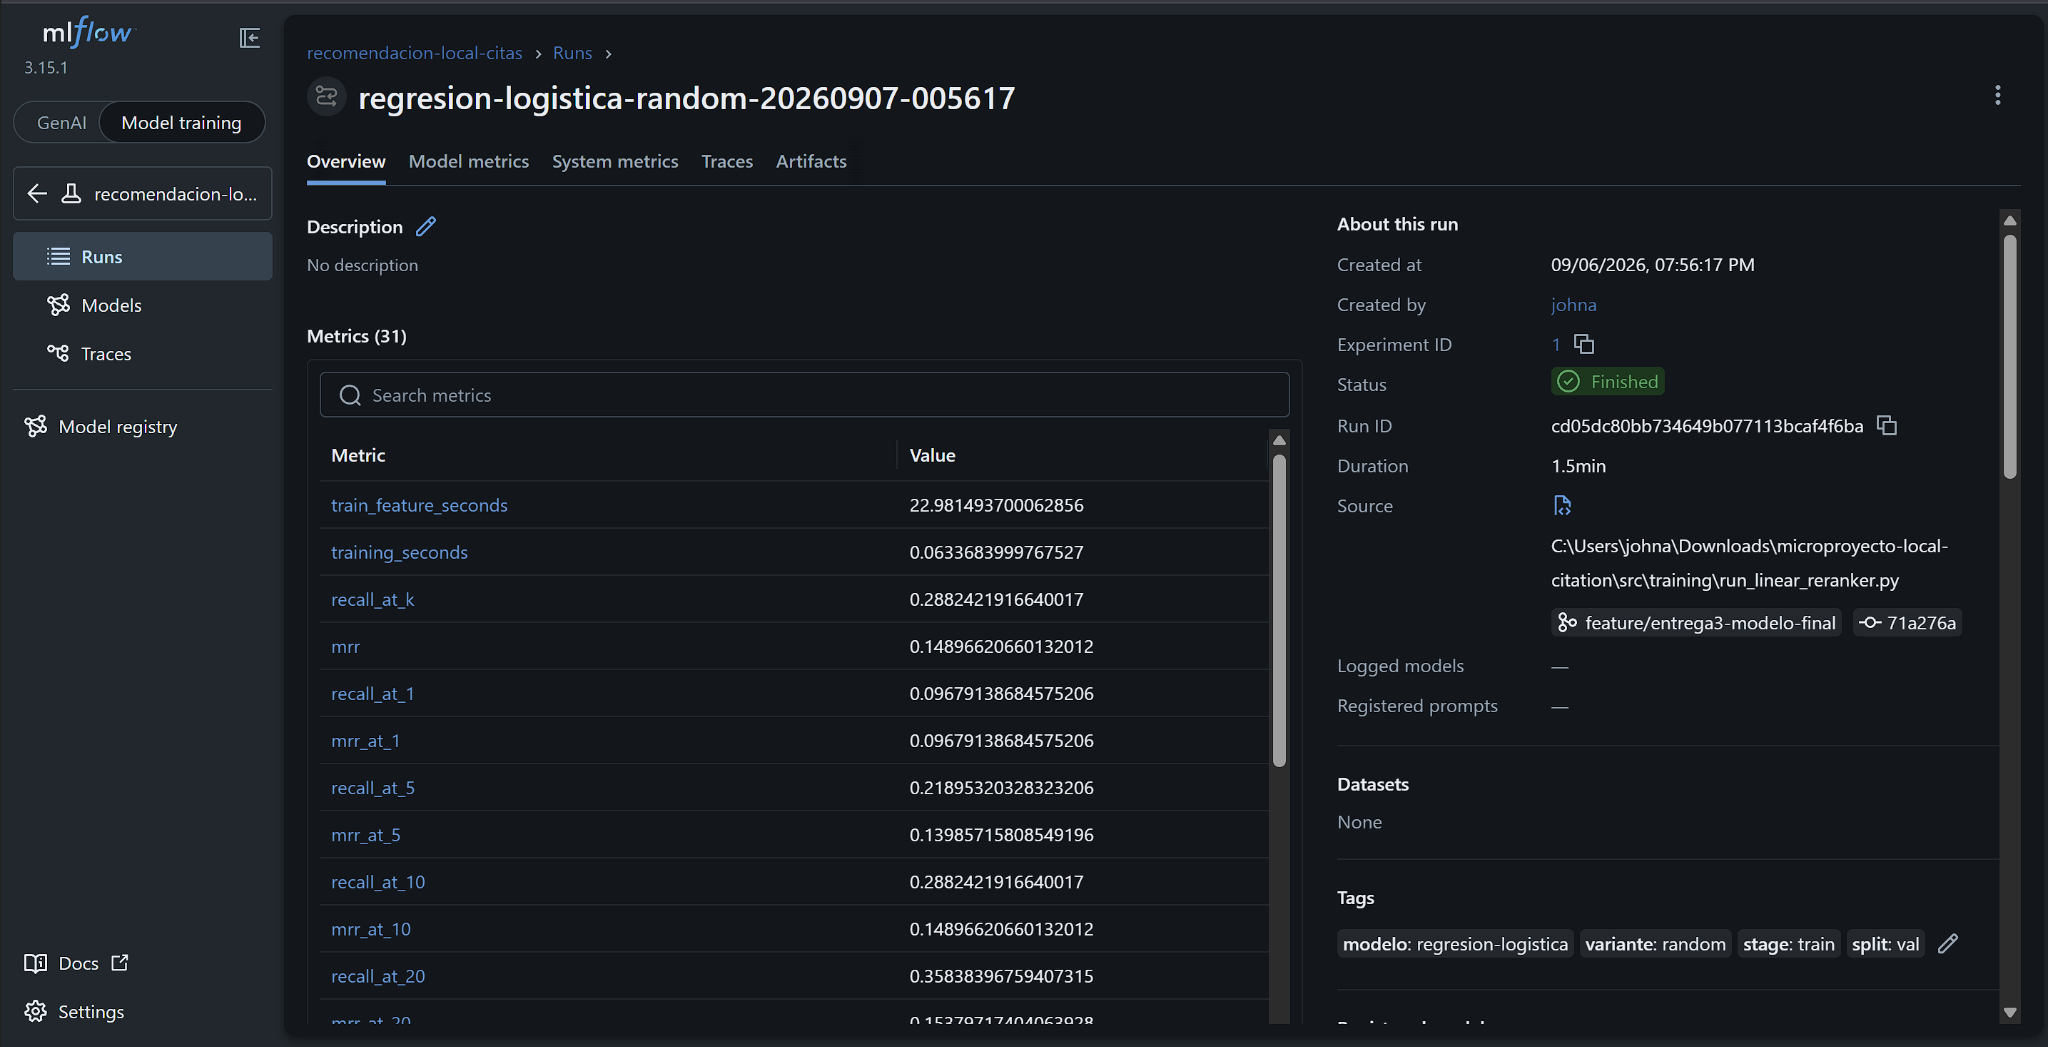
\includegraphics[width=\linewidth]{mlflow_run_random_detalle.png}
\caption*{(a) Detalle de la corrida Random}
\end{minipage}
\hfill
\begin{minipage}{0.49\textwidth}
\centering
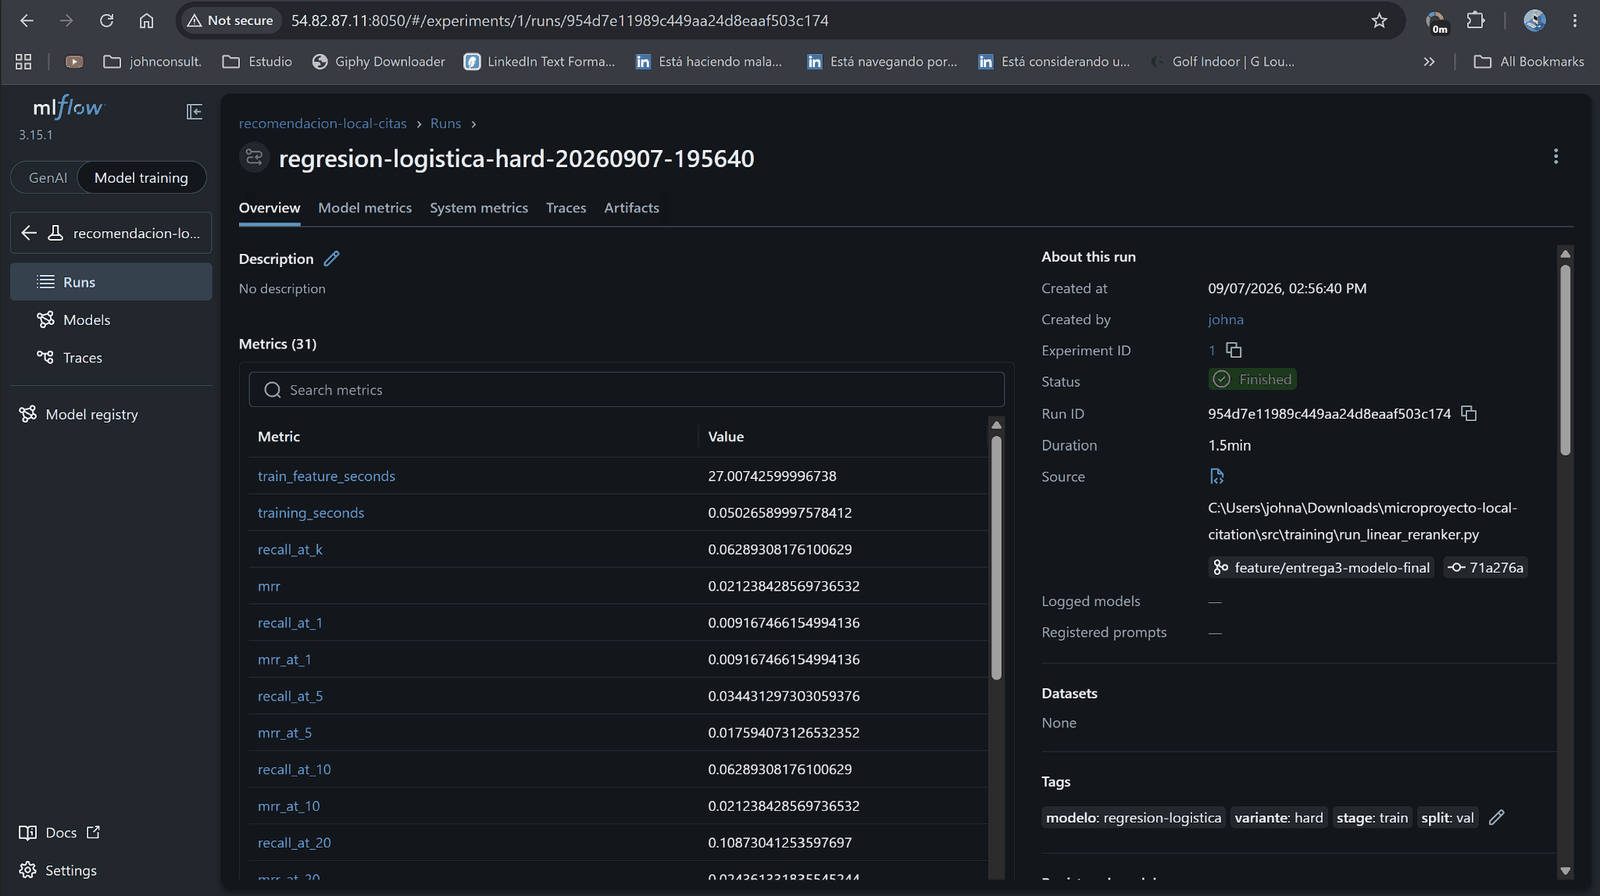
\includegraphics[width=\linewidth]{mlflow_run_hard_detalle.png}
\caption*{(b) Detalle de la corrida Hard}
\end{minipage}

\caption{Detalle de las dos variantes de entrenamiento almacenadas en MLflow.}
\end{figure}

El uso de MLflow permitió comparar las dos variantes sobre una misma base y
conservar evidencia de los resultados utilizados para escoger la configuración
final del modelo.

% ============================================================================
% 5. AWS
% ============================================================================

\section{MLflow en AWS}

Para que el seguimiento de experimentos no dependiera de una sola máquina
local, se instaló MLflow 3.15.1 en una instancia EC2 de AWS Academy con Ubuntu
24.04 LTS.

La instancia utiliza SQLite para guardar los metadatos de MLflow y un
directorio local para los artefactos. El servicio escucha por el puerto 8050 y
se configuró con \texttt{systemd} para que vuelva a iniciarse automáticamente
cuando la máquina arranque.

Uno de los inconvenientes encontrados durante el trabajo con AWS Academy fue
el cambio de la dirección IP pública después de detener y volver a iniciar la
instancia. Para evitar tener que actualizar esta dirección manualmente cada vez,
se creó el script \texttt{scripts/conectar\_mlflow\_aws.ps1}.

El script consulta la IP pública actual mediante AWS CLI, configura
\texttt{MLFLOW\_TRACKING\_URI} y comprueba que el puerto 8050 sea accesible
desde el equipo local.

Las siguientes imágenes muestran el servicio funcionando en EC2 y la conexión
automática desde PowerShell.

\begin{figure}[H]
\centering

\begin{minipage}{0.49\textwidth}
\centering
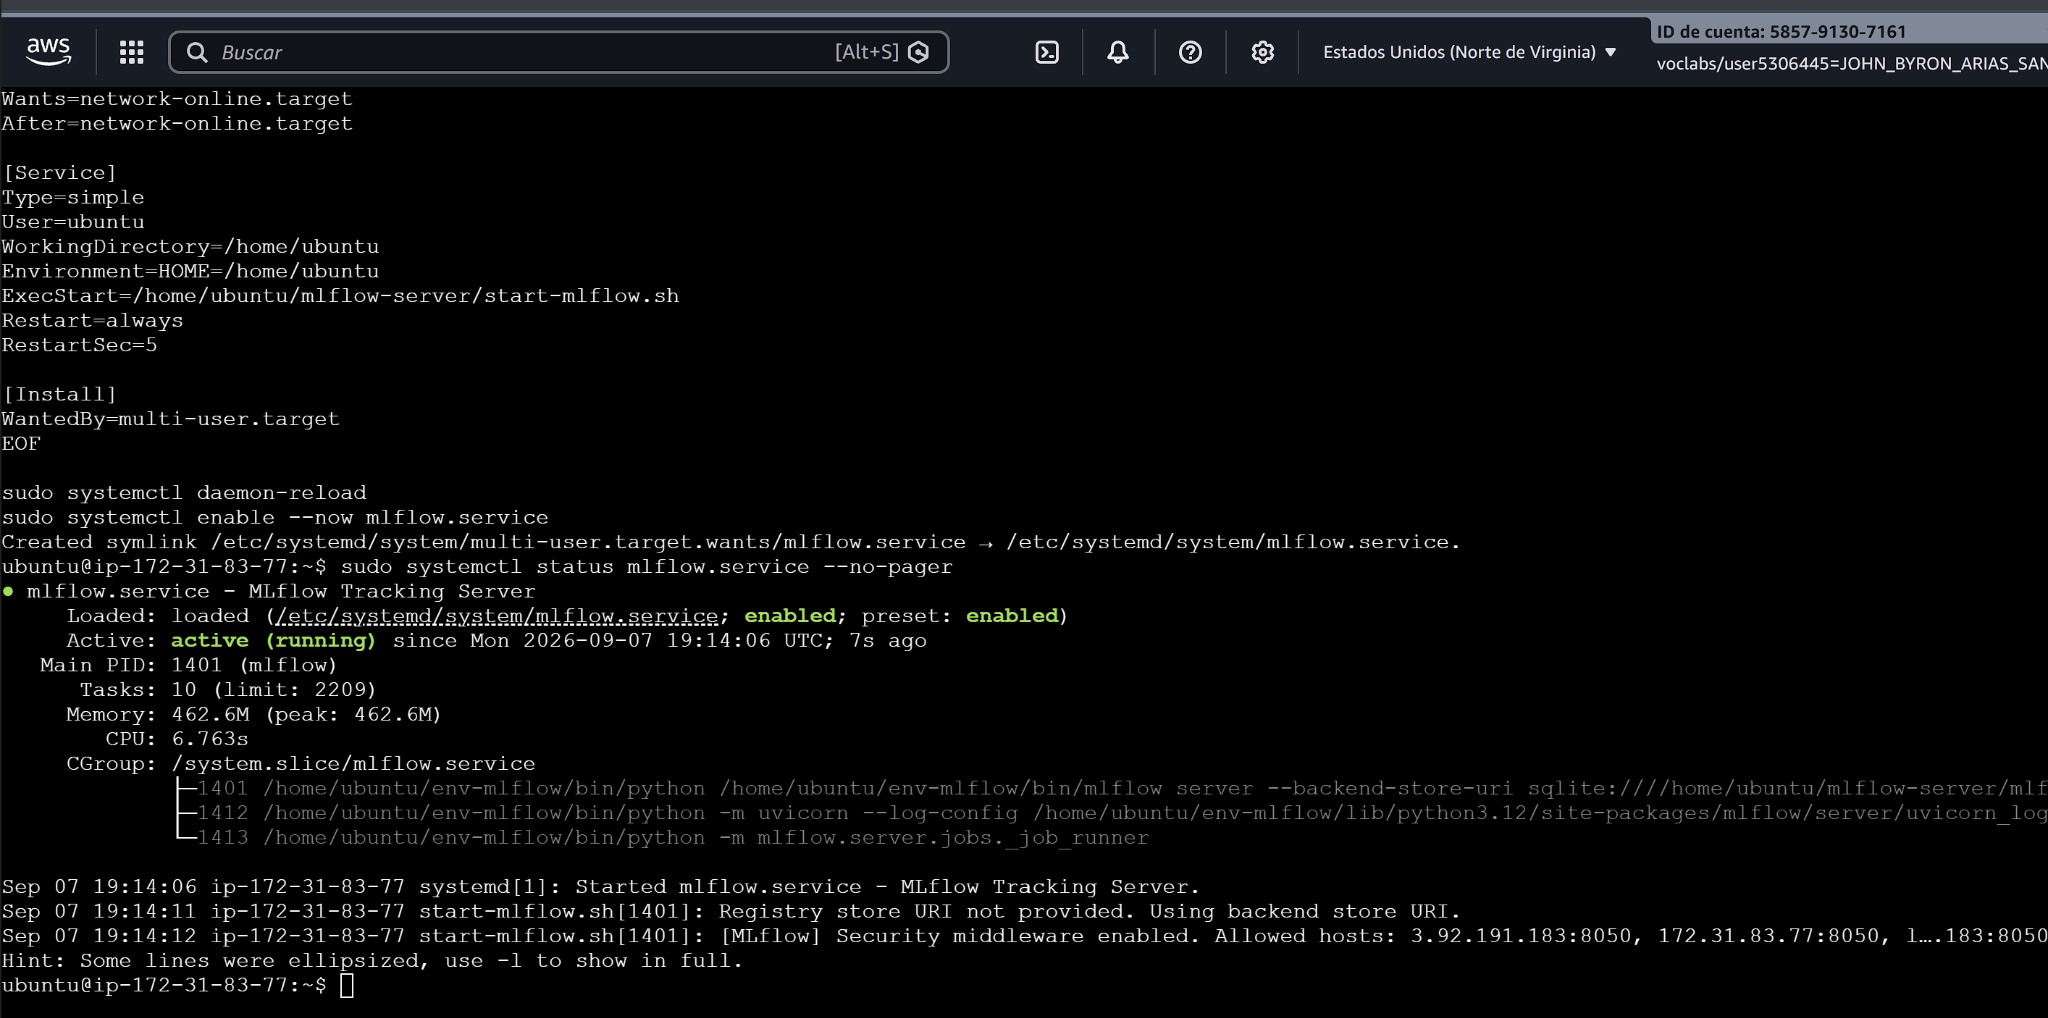
\includegraphics[width=\linewidth]{aws_mlflow_servicio_activo.png}
\caption*{(a) Servicio MLflow activo en EC2}
\end{minipage}
\hfill
\begin{minipage}{0.49\textwidth}
\centering
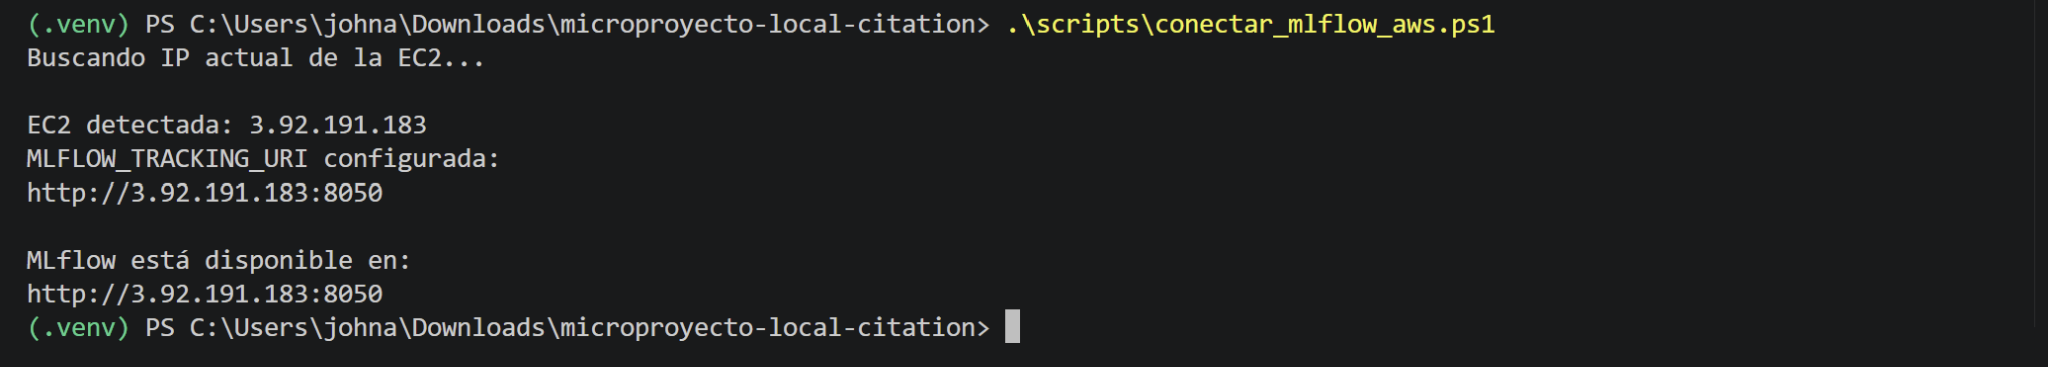
\includegraphics[width=\linewidth]{mlflow_conexion_aws_automatica.png}
\caption*{(b) Detección de la IP y conexión desde el equipo local}
\end{minipage}

\caption{Funcionamiento de la infraestructura de MLflow en AWS.}
\end{figure}

% ============================================================================
% 6. EMPAQUETAMIENTO
% ============================================================================

\section{Empaquetamiento e integración del modelo}

Otro avance de esta entrega fue convertir el recomendador en una librería
Python instalable. El código de desarrollo y entrenamiento permanece en
\texttt{model-package/}, pero la capa de producción consume
\texttt{modelo-citas} como un wheel versionado. La versión utilizada actualmente
es la 0.2.0, publicada en un bucket S3 de solo lectura y fijada por URL y hash
en \texttt{pyproject.toml} y \texttt{uv.lock}.

El wheel incluye el recuperador TF--IDF, el reordenador lineal, la
configuración, el modelo entrenado y la información necesaria para generar las
recomendaciones. En el artefacto 0.2.0 actualmente publicado,
\texttt{include\_metadata=false}; por ello el runtime sirve la variante v1
\texttt{Random} de cinco características. La variante v2 permanece como mejor
resultado experimental, pero no se presenta en este reporte como ya desplegada.
Por esta separación, FastAPI y las imágenes Docker no necesitan entrenar el
modelo, copiar \texttt{model-package/} ni descargar el dataset para servir
inferencias.

La interfaz pública del paquete puede utilizarse de esta forma:

\begin{verbatim}
from modelo_citas import make_prediction

resultado = make_prediction(
    context="Recent work on neural machine translation with attention",
    top_k=5,
)
\end{verbatim}

La validación posterior al refactor comprobó la frontera de producción:
\texttt{uv sync} instaló \texttt{modelo-citas} 0.2.0 desde S3 y Docker construyó
la API sin copiar \texttt{model-package/}, sin descargar el dataset y sin
reentrenar. También se ejecutaron las pruebas del paquete y la suite completa
del proyecto.

\notabox{
\textbf{Resultado de la validación posterior al refactor: 202 pruebas aprobadas.}

La suite completa se ejecutó con el grupo de dependencias de investigación y no
produjo fallos funcionales. Se observaron advertencias de deprecación asociadas
con NumPy/Joblib, pero no impidieron la ejecución actual.
}

% ============================================================================
% 7. API Y TABLERO
% ============================================================================

\section{API y tablero}

El paquete \texttt{modelo-citas} se integró con el backend desarrollado en
FastAPI. Al iniciar la aplicación, el backend carga el modelo empaquetado y
queda disponible para responder las consultas enviadas desde la API o desde el
tablero.

Los endpoints principales son:

\begin{center}
\footnotesize
\begin{tabular}{lll}
\toprule
\textbf{Método} & \textbf{Ruta} & \textbf{Función} \\
\midrule
GET  & \texttt{/api/estado} & Estado del modelo \\
POST & \texttt{/api/recomendar} & Generar recomendaciones \\
GET  & \texttt{/api/insights} & Información analítica \\
GET  & \texttt{/api/ejemplo} & Ejemplo real del corpus \\
GET  & \texttt{/docs} & Documentación Swagger/OpenAPI \\
\bottomrule
\end{tabular}
\end{center}

Las pruebas realizadas desde Swagger devolvieron código HTTP 200 y resultados
reales para el endpoint de recomendación. El endpoint
\texttt{/api/estado} confirmó que el paquete cargado es
\texttt{modelo-citas} 0.2.0 sobre un catálogo de 19.776 artículos. La ficha
técnica expuesta por ese endpoint reporta cinco coeficientes del reordenador,
coherentes con la variante v1 \texttt{Random} actualmente empaquetada.

El tablero se encuentra en \texttt{src/app/}. Desde la interfaz, el usuario
puede escribir un contexto, escoger cuántas recomendaciones desea recibir y
consultar el ranking generado. Al seleccionar un artículo también puede revisar
su resumen.

Además del recomendador, la interfaz presenta tres apartados de análisis:
estudio de los datos, desempeño del modelo y diagnóstico de negativos. Así,
desde una misma interfaz es posible probar el recomendador y consultar
información sobre los datos y el desempeño obtenido durante los experimentos.

% ============================================================================
% 8. USO E INSTALACION
% ============================================================================

\section{Uso, instalación y reproducibilidad}

\subsection{Uso del prototipo}

El flujo para utilizar el tablero es el siguiente:

\begin{enumerate}
    \item abrir la aplicación en el navegador;
    \item escribir o pegar un fragmento académico en inglés;
    \item escoger el número de recomendaciones;
    \item pulsar \textit{Recomendar citas};
    \item revisar los artículos recuperados y sus resúmenes.
\end{enumerate}

También puede utilizarse la opción \textit{Usar un ejemplo real} para cargar
una consulta conocida del conjunto de datos y observar el comportamiento del
recomendador.

Los resultados deben entenderse como apoyo a la búsqueda bibliográfica. La
pertinencia de una referencia debe revisarse antes de utilizarla en un documento
académico.

\subsection{Instalación}

El flujo principal para preparar el proyecto es:

\begin{verbatim}
git clone https://github.com/Byron971/microproyecto-local-citation.git
cd microproyecto-local-citation
docker compose up --build
\end{verbatim}

Con Docker Compose, los puntos de acceso son:

\begin{itemize}[leftmargin=1.4em, itemsep=0pt, topsep=1pt]
  \item tablero: \url{http://localhost:8080};
  \item estado de la API: \url{http://localhost:8000/api/estado};
  \item Swagger/OpenAPI: \url{http://localhost:8000/docs}.
\end{itemize}

El build instala directamente el wheel \texttt{modelo-citas} 0.2.0; no ejecuta
DVC ni entrenamiento.

Para reproducir experimentos, datos y pruebas se utiliza el grupo
\texttt{research}:

\begin{verbatim}
uv sync --group research
uv run --group research dvc pull
uv run --group research pytest
\end{verbatim}

La reproducibilidad del proyecto se apoya en Git y GitHub para el código, DVC
para los datos de investigación, MLflow para los experimentos, uv para las
dependencias y pytest/Tox para las pruebas. La capa de producción queda
desacoplada del entrenamiento mediante el wheel versionado.

% ============================================================================
% 9. ESTADO
% ============================================================================

\section{Estado al cierre de la Entrega 3}

Al cierre de este reporte se encuentran implementados los componentes de datos,
experimentación, empaquetamiento, API, tablero y contenedores. El estado se
presenta separando explícitamente la mejor variante experimental del modelo que
se encuentra empaquetado y demostrado en la API.

\begin{table}[H]
\centering
\footnotesize

\begin{tabular}{p{9cm}p{3cm}}
\toprule
\textbf{Componente} & \textbf{Estado} \\
\midrule
Repositorio Git y colaboración & Realizado \\
Datos versionados con DVC & Realizado \\
Modelos y comparación experimental & Realizado \\
Seguimiento con MLflow & Realizado \\
Mejor variante experimental (v2 Random) & Realizado \\
Modelo empaquetado (v1 Random, wheel 0.2.0) & Realizado \\
API con modelo empaquetado & Realizado \\
Tablero integrado & Realizado \\
Pruebas automatizadas & 202 pruebas aprobadas \\
Manual de usuario e instalación & Actualizado \\
Dockerización & Realizado \\
Despliegue mediante contenedores & Realizado \\
Evidencia de despliegue en AWS & Previa al refactor final \\
Validación post-refactor & Local con Docker Compose \\
Video final & Pendiente \\
Reporte final de aportes & Realizado \\
\bottomrule
\end{tabular}

\caption{Estado de los componentes al cierre de la Entrega 3.}
\end{table}

Después del refactor de responsabilidades se repitió la validación del sistema.
La suite completa finalizó con 202 pruebas aprobadas. En Windows 11, Docker
Desktop sobre WSL2 construyó y levantó los servicios con
\texttt{docker compose up --build}, y el healthcheck de la API respondió
correctamente. El endpoint \texttt{/api/estado} reportó
\texttt{listo=true}, paquete \texttt{modelo-citas} 0.2.0 y 19.776 artículos.
Desde \texttt{localhost:8080} se cargó un ejemplo real y el tablero devolvió un
ranking de recomendaciones con sus resúmenes. Esta validación confirma la
arquitectura de producción posterior al refactor, pero no implica que la
variante v2 experimental ya esté publicada en el wheel. El procedimiento
actualizado se encuentra en \texttt{docs/manual\_instalacion.md}.

\pendingbox{
Para cerrar la entrega queda grabar y publicar el video de síntesis e incorporar
su enlace. Si el equipo decide que la variante v2 debe ser también la versión
servida, será necesario publicar un nuevo wheel con
\texttt{include\_metadata=true} y repetir la validación de Docker. Mientras eso
no ocurra, este reporte diferencia explícitamente entre v2 experimental y v1
desplegada.
}

\notabox{
\textbf{Soportes principales de la entrega:}
repositorio GitHub \url{https://github.com/Byron971/microproyecto-local-citation};
datos en \texttt{data/raw.dvc} y \texttt{data/processed.dvc};
manuales en \texttt{docs/manual\_usuario.md} y
\texttt{docs/manual\_instalacion.md}; artefactos de contenedores
\texttt{Dockerfile}, \texttt{Dockerfile.dashboard} y
\texttt{docker-compose.yml}; evidencias de MLflow y despliegue en
\texttt{reportes/reporte03/}.
}

% ============================================================================
% 10. EQUIPO
% ============================================================================

\section{Trabajo en equipo}

El trabajo se ha organizado mediante ramas, issues, commits y Pull Requests.
Los cambios de mayor impacto se revisan antes de incorporarse a
\texttt{main}. El repositorio también cuenta con \texttt{CODEOWNERS}, lo que
permite solicitar revisión a otros integrantes antes de aceptar determinados
cambios.

Durante esta fase se revisó la integración final del modelo y el refactor que
separó entrenamiento y producción. El código de investigación quedó en
\texttt{model-package/}, mientras la API instala un wheel versionado desde S3.
Después del refactor se ejecutaron 202 pruebas y se validó el flujo
Docker $\rightarrow$ API $\rightarrow$ modelo $\rightarrow$ tablero mediante
una recomendación real. La revisión también permitió identificar que el wheel
0.2.0 mantiene la configuración v1 de cinco características, mientras v2 sigue
siendo la mejor variante experimental.

\begin{table}[H]
\centering
\scriptsize

\begin{tabular}{p{2.5cm}p{10.6cm}}
\toprule
\textbf{Integrante} & \textbf{Aportes principales} \\
\midrule

John Arias &
Comparación Random vs. Hard y evidencias de MLflow; automatización de conexión
a MLflow en AWS; preparación reproducible de DVC; integración del tablero con
la API; dockerización de API y tablero, Docker Compose y documentación del
despliegue en AWS; manual de usuario y consolidación del reporte. Para el corte
del 20 de septiembre coordinó además la evaluación global, integró el pipeline
de métricas, los clientes de modelos comerciales/open-weight y realizó la
primera validación manual por parte del equipo sobre 20 casos piloto. \\

Carlos Duque &
Desarrollo de la maqueta inicial en HTML y FastAPI; implementación de una
aplicación para servir el tablero y predicciones; empaquetamiento del modelo
como \texttt{modelo-citas}; construcción del paquete instalable y refactor
final para separar entrenamiento y producción. Esta última arquitectura
publica el modelo como wheel versionado en S3 y permite que FastAPI y Docker lo
consuman sin copiar \texttt{model-package/}, sin DVC y sin entrenar durante el
build. \\

José Zambrana &
Desarrollo del reordenador supervisado, extracción de características,
regresión logística, generación de negativos difíciles, evaluación mediante
Recall@K y MRR y documentación de resultados; apoyo en DVC y actualización de
evidencias de MLflow. También diseñó y versionó los tres prompts de función de
cita (zero-shot genérico, zero-shot detallado y few-shot), el conjunto piloto y
el análisis de estabilidad y errores de formato. \\

Carlos Caicedo &
Desarrollo y evaluación de la línea base TF--IDF; configuración inicial de
MLflow y remotos DVC; diagnóstico de negativos; implementación y evaluación del
reordenador versión 2 con características de metadatos; documentación del
modelo final; creación y verificación del manual de instalación y auditoría
desde entorno limpio, incluida evidencia de Docker y despliegue. \\

\bottomrule
\end{tabular}

\caption{Resumen de los aportes realizados durante la Entrega 3.}
\end{table}

La tabla resume contribuciones verificables en el historial del repositorio,
issues y Pull Requests. De acuerdo con la guía del curso, la contribución
individual se respalda mediante commits, el reporte de trabajo en equipo y la
sustentación; el video puede apoyarse en esta distribución para presentar el
trabajo realizado.

Como extensión adicional se versionaron tres estrategias de \emph{prompting},
el parser común de nueve puntajes y el pipeline de métricas con Precision,
Recall, F1 Macro/Micro y matrices de confusión. Se completó una primera
validación manual sobre 20 casos piloto y se ejecutaron corridas provisionales
con Qwen3:8B, Gemini y Cohere; OpenAI quedó implementado, pero sin predicciones
por falta de saldo disponible. El detalle se conserva en
\texttt{docs/evaluacion\_comparativa\_provisional\_20sep.md}.

Posteriormente se completó la segunda validación humana independiente sobre los
mismos 20 casos, realizada sin consultar la primera hoja ni las sugerencias
automáticas. El acuerdo fue de 12 coincidencias y 8 desacuerdos, es decir una
tasa de 0,60 y un \emph{Cohen Kappa} de 0,4839, valor que corresponde a un
acuerdo moderado y se ubica dentro del rango habitual para taxonomías de función
de cita con nueve clases. Tras reconciliar los desacuerdos quedó congelado el
\emph{Test Gold} definitivo en
\texttt{annotations/citation\_function/test\_gold.jsonl}, que difiere del
conjunto provisional en un único caso.

Tres limitaciones acompañan esa cifra. Primero, el Kappa compara una anotación
asistida con explicaciones contra una independiente, no dos anotaciones ciegas.
Segundo, la reconciliación de los ocho desacuerdos también fue asistida, y siete
se resolvieron hacia la etiqueta del primer anotador. Tercero, el conjunto
definitivo cubre solo 5 de las 9 categorías ---Background, Application,
Evidence, Improvement y Further Reading---, por lo que el F1 Macro sobre las
nueve clases permanece penalizado por las cuatro ausentes; ampliar el piloto más
allá de 20 casos es la vía para levantar esa restricción. Las corridas de los
modelos sobre este conjunto definitivo quedan pendientes.

% ============================================================================
% 11. CONCLUSIONES
% ============================================================================

\section{Conclusiones}

La comparación experimental identificó a la versión 2 con negativos aleatorios
como la mejor variante medida: alcanzó Recall@10 de 0,3793 y MRR@10 de 0,2166,
mientras que la versión 2 con negativos difíciles obtuvo 0,2288 y 0,0995. Sin
embargo, la versión actualmente empaquetada y demostrada en la API es v1
\texttt{Random}, incluida en \texttt{modelo-citas} 0.2.0. Esta distinción evita
atribuir al sistema desplegado métricas que corresponden a una variante todavía
no publicada en el wheel.

El experimento también permitió identificar una limitación importante. Con
Recall@100 de 0,5160, cerca del 48,4\,\% de las consultas de validación no tiene
la cita correcta dentro de los cien candidatos iniciales. Por ello, además de
mejorar el reordenador, una línea prioritaria de trabajo es fortalecer la etapa
de recuperación.

Además de mejorar el modelo, durante esta entrega se avanzó en la construcción
de una solución que pueda reproducirse y reutilizarse fuera del entorno de
experimentación. Los datos están versionados con DVC, los experimentos quedan
registrados en MLflow, el modelo puede instalarse como wheel y ya es consumido
por FastAPI y por el tablero.

La contenerización quedó completada y verificada después del refactor. La
imagen de la API instala el wheel \texttt{modelo-citas} 0.2.0 publicado en S3 y
no incorpora dependencias de entrenamiento ni necesita descargar los datos
durante el build. La arquitectura final fue validada localmente con Docker
Compose, API saludable y una recomendación real desde el tablero. Las evidencias
en AWS corresponden al despliegue realizado antes del refactor final y se
conservan como soporte histórico de la Entrega 3.

Para cerrar la Entrega 3 queda pendiente el video de síntesis y su enlace final.
Si se desea desplegar también la mejor variante experimental, el siguiente paso
es publicar un nuevo wheel con v2 y repetir la prueba contenerizada. En la
extensión de clasificación de función de cita ya se completaron la segunda
validación humana independiente, el cálculo de acuerdo y la reconciliación, con
un Cohen Kappa de 0,4839; resta repetir la evaluación de los modelos sobre el
Test Gold definitivo antes de presentar esos resultados como definitivos. En el recomendador principal, el Recall@100 de
0,5160 muestra que un margen importante de mejora está en la recuperación de
candidatos, por ejemplo mediante representaciones semánticas más ricas.

% ============================================================================
% REFERENCIAS
% ============================================================================

\section*{Referencias}

\scriptsize

Gu, N. (2022).
\textit{Local-Citation-Recommendation} [Computer software].
GitHub.
\url{https://github.com/nianlonggu/Local-Citation-Recommendation}

Gu, N., Gao, Y., \& Hahnloser, R. H. R. (2022).
Local citation recommendation with hierarchical-attention text encoder and
SciBERT-based reranking.
\textit{Advances in Information Retrieval}, 274--288.
Springer.
\url{https://doi.org/10.1007/978-3-030-99736-6_19}

Treveil, M., \& Dataiku Team. (2021).
\textit{Introducing MLOps: How to scale machine learning in the enterprise}.
O'Reilly Media.

\end{document}